\section{Fluidos y flujo de fluidos}

¿Qué es un fluido? Un fluido es una sustancia que se deforma continuamente cuando se le somete a un esfuerzo cortante, sin importar lo pequeño que sea el esfuerzo aplicado. Este concepto engloba tanto a,

\begin{itemize}
\item los \emph{líquidos}, los cuales toman la forma del recipiente que los aloja y mantienen su volumen
\item los \emph{gases}, los cuales carecen de volumen como de forma propia
\end{itemize}

\begin{figure}
  \begin{figurebox}
    \vspace{20pt}
    \centering
\begin{subfigure}{.3\textwidth}
  \centering
   \includegraphics[height=100pt]{fig1.jpg}
   \caption{Pelìcula de jabón iluminada}
  \label{fig:0a} 
\end{subfigure}%
\begin{subfigure}{.3\textwidth}
  \centering
  \includegraphics[height=100pt]{fig2.jpg}
  \caption{Desplazamiento de viscosidad}
  \label{fig:0b}
\end{subfigure}
\begin{subfigure}{.3\textwidth}
  \centering
  \includegraphics[height=100pt]{fig3.jpg}
  \caption{Burbujas en detergente puro}
  \label{fig:0c}
\end{subfigure}
\caption{Imágenes de comportamiento de fluidos extraidas de \cite{linkfluids}}
\label{fig:test}
  \end{figurebox}
\end{figure}

El estudio del movimiento de un fluido es lo que llamamos mecánica de fluidos. El flujo  se define como el movimiento de un fluido. El estudio del  flujo,  es muy complejo y no es lo mismo estudiar el fluido del agua, el fluído de la miel, el fluido de la sangre o el comportamiento del humo de un cigarro. Nosotros en este artículo nos vamos a centrar en fluidos que se denominan {\em fluidos ideales}. Consideramos el comportamiento de un fluido ideal cuyas características son las siguientes:

\begin{itemize}

\item \emph{No viscoso:} esto significa que se desprecia la fricción interna entre las distintas partes del fluido. Piensa: ¿Qué es más viscoso la miel o el agua?

\item \emph{Estado estacionario:}  esto es que la velocidad del fluido en un punto es constante con el tiempo. Estos se caracterizan por las siguientes propiedades:

\item \emph{Incompresible:} la densidad del fluido permanece constante con el tiempo.

\item \emph{Irrotacional:} no presenta torbellinos, es decir, no hay momento angular del fluido respecto de cualquier punto. Es decir, cada partícula del fluido sigue una trayectoria uniforme y estas no se cruzan. Piensa: ¿es el humo de un cigarro  un fluído irrotacional?

\end{itemize}

%\begin{wrapfigure}{r}{0.7\textwidth} 
%\vspace{-1.2cm}
%  \begin{mybox}
%    Otra clasificación:\emph{fluidos newtonianos y no newtonianos} proviene de la palabra \emph{catena},
%    que significa \emph{cadena} en Latín Un fluido newtoniano es un fluido cuya viscosidad puede considerarse constante en el tiempo. El mejor ejemplo de este tipo de fluidos es el agua en contraposición al pegamento, la miel o los geles y sangre que son ejemplos de fluidos no newtonianos.
%\end{mybox}
%\vspace{-1cm}
%\end{wrapfigure}


Fluídos ideales puros en la realidad no existen pero si podemos despreciar esas diferencias y poder tomar algunos líquidos y gases como fluídos ideales. El ejemplo más cercano a fluído ideal es el agua. En particular, vamos a estudiar algunos detalles del estudio de flujos por el interior de tuberías como son el conocimiento del caudal y la velocidad del fluido que circula a través de una tubería.


Algunas curiosidades de la complejidad que presentan los fluidos y el flujo de fluidos son:
\begin{itemize}
\item Revelaron que en ausencia de gravedad los líquidos se convierten en algo más viscoso que tiende a unirse en una sola bola con una gran tensión superficial. Y que si colocamos al lado una burbuja de agua más pequeña, la bola grande la absorbe rápidamente, como si fuera un imán.

\item El estudio de fluidos es algo complejo, pero tambièn podemos verlo como algo artìstico. Véase la Figura 1.

\end{itemize}
\section{Ecuación de Continuidad}

Cuando echamos agua por un lado de un tubo hueco y abierto por ambos lados, sabemos que algo va a pasar, ¿verdad? El agua va a salir por el otro lado. Da igual si el tubo tiene diámetro constante o si cambia, el caudal que entra por un lado va a salir por el otro.  Esto es lo que se llama en mecánica de fluidos la Ecuación de Continuidad. Esta ecuación no es más que un caso particular del principio de conservación de la masa (véase \cite{white}). Vamos a verla.

Vamos a referir a la Figura \ref{fig:2} para entender mejor el razonamiento que vamos a llevar a cabo. 


\begin{figure}[h!] 
\begin{figurebox}
      \centering
    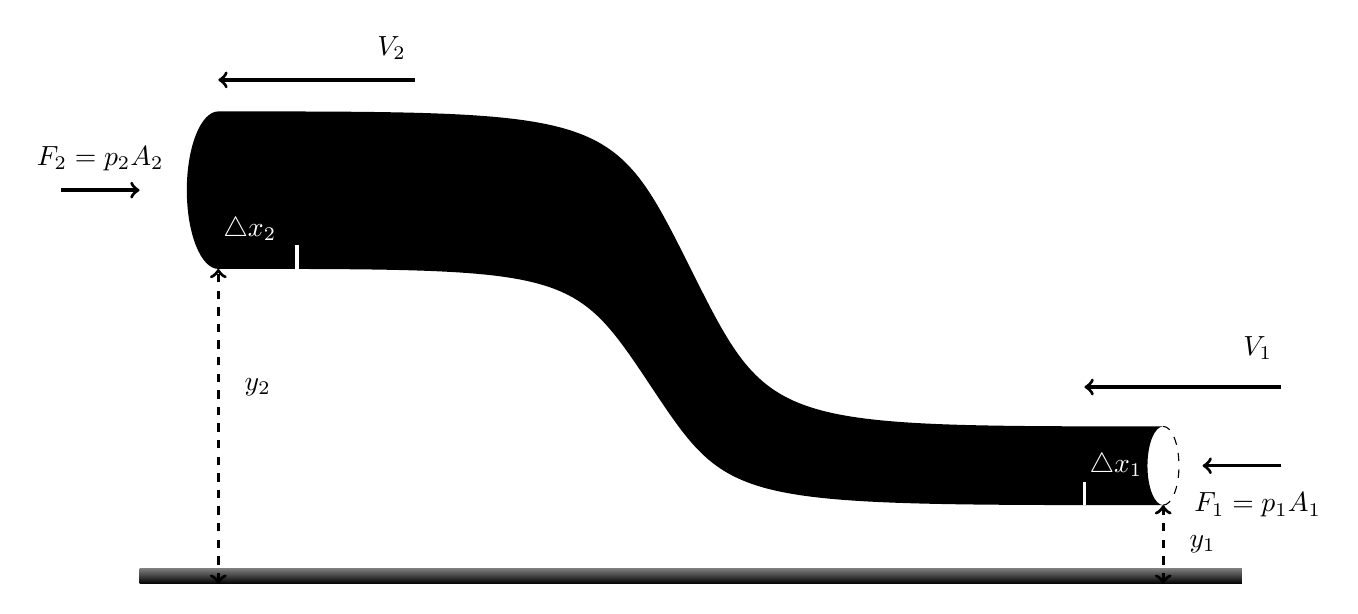
\begin{tikzpicture}
      \shade[top color=gray, bottom color=black] (-1,-2) rectangle +(14,0.2);

      \fill[black] (0,4) .. controls (5,4) .. (6,2)
      .. controls (7,0) .. (12,0)
      arc (90:270:0.2 and 0.5)
      .. controls (6.5,-1) .. (5.5,0.5)
      .. controls (4.5,2) .. (0,2)
      arc (270:90:0.4 and 1) -- cycle;
      \draw[dashed] (12,-1) arc (-90:90:0.2 and 0.5);

      \draw[<-,very thick] (12.5,-0.5)--(13.5,-0.5);
      \draw [black] (13.2,-1) node {$F_1=p_1 A_1$};
      \draw[<-,very thick] (11,0.5)--(13.5,0.5);
      \draw [black] (13.2,1) node {$V_1$};
      \draw[<->,very thick,dashed] (12,-2) --(12,-1);
      \draw [black] (12.5,-1.5) node {$y_1$};
      \draw[very thick,white] (11,-1)--(11,-0.7);
      \draw [white,very thick] (11.4,-0.5) node {$\triangle x_1$}; 

      \draw[->,very thick] (-2,3)--(-1,3);
      \draw [black] (-1.5,3.4) node {$F_2=p_2 A_2$};
      \draw[<-,very thick] (0,4.4)--(2.5,4.4);
      \draw [black] (2.2,4.8) node {$V_2$};
      \draw[very thick,white] (1,2)--(1,2.3);
      \draw [white,very thick] (0.4,2.5) node {$\triangle x_2$}; 
      \draw[<->,very thick,dashed] (0,-2) --(0,2);
      \draw [black] (0.5,0.5) node {$y_2$}; 
      
    \end{tikzpicture}
  \caption{Fluido en movimiento en un tubo}
  \label{fig:2}
  \end{figurebox}
\end{figure}


%\begin{wrapfigure}{r}{0.5\textwidth} 
%  \begin{figurebox}
%  \centering
%  \includegraphics[width=\textwidth]{Tuberia1.png}
%  \caption{Hilos con distintos longitudes.}
%  \label{fig:2}
%\end{figurebox}
%\end{wrapfigure}

Consideramos un fluido que se mueve a lo largo de un tubo, cuya sección transversal aumenta en dirección del flujo, como en la Figura \ref{fig:2}. En un intervalo de tiempo que vamos a llamar $\triangle t$,  en la sección más angosta del tubo de área $A_1$, el fluido se mueve una distancia $\triangle_1= V_1  \cdot \triangle t$ siendo $V_1$ la velocidad del fluido. La masa contenida en el volumen $A_1 \cdot \triangle_1$  es $m_1=\rho_1 \cdot A_1 \cdot \triangle x_1$ siendo $\rho_1$ la densidad del fluido en ese intervalo de tiempo. De manera similar, en la seccion ancha del tubo de área $A_2$, se obtienen expresiones equivalentes en el mismo intervalo de tiempo $\triangle t$, cambiando el subindice 1 por 2. Pero la masa se conserva en el flujo estacionario, esto es la masa que cruza por $A_1$ es igual a la masa que pasa por $A_2$ en el intervalo de tiempo $\triangle t$. De este modo tenemos la ecuación de Continuidad como sigue:

\begin{equation} 
\rho_1 \cdot A_1\cdot  V_1=\rho_1\cdot  A_2 \cdot V_2
\end{equation}

Si estamos en un fluido incomprensible esta ecuación se reduce a:

\begin{equation}\label{EqContinuidad} 
A_1\cdot  V_1=A_2\cdot  V_2=constante.
\end{equation}

La cantidad $A\cdot V$ se llama flujo de volumen o caudal. Y, ¿qué podemos deducir de esta ecuación? Que a mayor sección, menor velocidad. Es decir, mirando en la Figura \ref{fig:2}, ¿por donde irá el agua más deprisa, en la parte angosta o en la parte más ancha?

Con esta simple ecuación podemos hacer un simple ejercicio. Si te fijas, ¿qué le pasa al agua cuando sale del grifo? El hilo de agua parece que es más fino cuánto más lejos del grifo, ¿verdad? Imaginemos que la boca del grifo es circular con un radio $r_0$,  Podemos ver como disminuye esa gota usando la ecuaciòn de continuidad. A la salida del grifo podemos suponer que la velocidad del agua es $V_0$. Por tanto el caudal a la salida del grifo es $V_0 \cdot \pi \cdot r_o^2$. la pregunta qué nos hacemos es, ¿cuál es el caudal a una distancia $h$ de la salida del grifo? 

 La velocidad del agua a esa distancia $h$ es $V_f$ y su valor se calcula como $$V_f^2=V_0²+\frac{1}{2}hg,$$ siendo $g$ la aceleración gravitatoria y por tanto el caudal a distancia $h$ del grifo es $\sqrt{V_0^2+\frac{1}{2} h g} \cdot \pi \cdot r^2 $ siendo $r$ el radio de la superficie del agua a esa altura. Y usando la ecuación de continuidad sabemos que el caudal es contante y por tanto, tenemos que
$$
V_0 \pi r_o^2=(V_0²+\frac{1}{2}hg) \pi r^2,
$$
y despejando la incógnita $r$, tenemos que 
\begin{equation}\label{eq:radio}
r=r_o \sqrt[4]{\frac{V_0^2}{V_0^2+\frac{1}{2}hg}}. 
\end{equation}

Usando octave podemos ver mejor la interpretación de la fórmula dada en la ecuación \ref{eq:radio}. Partiendo de datos iniciales la velocidad inicial (por ejemplo $V_0=3.2$ m/s), el radio del grifo (por ejemplo $r_0=0.05$ m), veamos como va la secciòn de la gota de agua segùn la distancia $h$ desde el grifo. 
\begin{octavebox}
\begin{verbatim}
g=9.81;V_0=3.2;r_0=0.05;
h=0:0.05:10;
r=r_0.*(V^2./(V^2+2*g*h)).^(1/4);
plot(h,rh)
title("Evoluciòn del radio del agua al salir de un grifo")
xlabel("h")
ylabel("r")
\end{verbatim}
\end{octavebox}

Y de esta manera obtenemos la gráfica en la Figura \ref{fig:3} en (a). Usando este radio también podemos dibujar las superficies de la gota de agua a diferentes alturas obteniendo la figura (b) de Figura \ref{fig:3}. ¿Te animas a dibujarlo tú en octave?


\begin{figure}
  \begin{figurebox}
    \vspace{20pt}
    \centering
\begin{subfigure}{.5\textwidth}
  \centering
   \scalebox{0.35}{ % GNUPLOT: LaTeX picture with Postscript
\begingroup
  \makeatletter
  \providecommand\color[2][]{%
    \GenericError{(gnuplot) \space\space\space\@spaces}{%
      Package color not loaded in conjunction with
      terminal option `colourtext'%
    }{See the gnuplot documentation for explanation.%
    }{Either use 'blacktext' in gnuplot or load the package
      color.sty in LaTeX.}%
    \renewcommand\color[2][]{}%
  }%
  \providecommand\includegraphics[2][]{%
    \GenericError{(gnuplot) \space\space\space\@spaces}{%
      Package graphicx or graphics not loaded%
    }{See the gnuplot documentation for explanation.%
    }{The gnuplot epslatex terminal needs graphicx.sty or graphics.sty.}%
    \renewcommand\includegraphics[2][]{}%
  }%
  \providecommand\rotatebox[2]{#2}%
  \@ifundefined{ifGPcolor}{%
    \newif\ifGPcolor
    \GPcolorfalse
  }{}%
  \@ifundefined{ifGPblacktext}{%
    \newif\ifGPblacktext
    \GPblacktexttrue
  }{}%
  % define a \g@addto@macro without @ in the name:
  \let\gplgaddtomacro\g@addto@macro
  % define empty templates for all commands taking text:
  \gdef\gplbacktext{}%
  \gdef\gplfronttext{}%
  \makeatother
  \ifGPblacktext
    % no textcolor at all
    \def\colorrgb#1{}%
    \def\colorgray#1{}%
  \else
    % gray or color?
    \ifGPcolor
      \def\colorrgb#1{\color[rgb]{#1}}%
      \def\colorgray#1{\color[gray]{#1}}%
      \expandafter\def\csname LTw\endcsname{\color{white}}%
      \expandafter\def\csname LTb\endcsname{\color{black}}%
      \expandafter\def\csname LTa\endcsname{\color{black}}%
      \expandafter\def\csname LT0\endcsname{\color[rgb]{1,0,0}}%
      \expandafter\def\csname LT1\endcsname{\color[rgb]{0,1,0}}%
      \expandafter\def\csname LT2\endcsname{\color[rgb]{0,0,1}}%
      \expandafter\def\csname LT3\endcsname{\color[rgb]{1,0,1}}%
      \expandafter\def\csname LT4\endcsname{\color[rgb]{0,1,1}}%
      \expandafter\def\csname LT5\endcsname{\color[rgb]{1,1,0}}%
      \expandafter\def\csname LT6\endcsname{\color[rgb]{0,0,0}}%
      \expandafter\def\csname LT7\endcsname{\color[rgb]{1,0.3,0}}%
      \expandafter\def\csname LT8\endcsname{\color[rgb]{0.5,0.5,0.5}}%
    \else
      % gray
      \def\colorrgb#1{\color{black}}%
      \def\colorgray#1{\color[gray]{#1}}%
      \expandafter\def\csname LTw\endcsname{\color{white}}%
      \expandafter\def\csname LTb\endcsname{\color{black}}%
      \expandafter\def\csname LTa\endcsname{\color{black}}%
      \expandafter\def\csname LT0\endcsname{\color{black}}%
      \expandafter\def\csname LT1\endcsname{\color{black}}%
      \expandafter\def\csname LT2\endcsname{\color{black}}%
      \expandafter\def\csname LT3\endcsname{\color{black}}%
      \expandafter\def\csname LT4\endcsname{\color{black}}%
      \expandafter\def\csname LT5\endcsname{\color{black}}%
      \expandafter\def\csname LT6\endcsname{\color{black}}%
      \expandafter\def\csname LT7\endcsname{\color{black}}%
      \expandafter\def\csname LT8\endcsname{\color{black}}%
    \fi
  \fi
  \setlength{\unitlength}{0.0500bp}%
  \begin{picture}(11520.00,8640.00)%
    \gplgaddtomacro\gplbacktext{%
    }%
    \gplgaddtomacro\gplfronttext{%
    }%
    \gplgaddtomacro\gplbacktext{%
    }%
    \gplgaddtomacro\gplfronttext{%
    }%
    \gplgaddtomacro\gplbacktext{%
      \colorrgb{0.00,0.00,0.00}%
      \put(7847,950){\makebox(0,0)[r]{\strut{}0.02}}%
      \colorrgb{0.00,0.00,0.00}%
      \put(7847,2124){\makebox(0,0)[r]{\strut{}0.025}}%
      \colorrgb{0.00,0.00,0.00}%
      \put(7847,3297){\makebox(0,0)[r]{\strut{}0.03}}%
      \colorrgb{0.00,0.00,0.00}%
      \put(7847,4471){\makebox(0,0)[r]{\strut{}0.035}}%
      \colorrgb{0.00,0.00,0.00}%
      \put(7847,5644){\makebox(0,0)[r]{\strut{}0.04}}%
      \colorrgb{0.00,0.00,0.00}%
      \put(7847,6817){\makebox(0,0)[r]{\strut{}0.045}}%
      \colorrgb{0.00,0.00,0.00}%
      \put(7847,7991){\makebox(0,0)[r]{\strut{}0.05}}%
      \colorrgb{0.00,0.00,0.00}%
      \put(7967,750){\makebox(0,0){\strut{}0}}%
      \colorrgb{0.00,0.00,0.00}%
      \put(8458,750){\makebox(0,0){\strut{}2}}%
      \colorrgb{0.00,0.00,0.00}%
      \put(8950,750){\makebox(0,0){\strut{}4}}%
      \colorrgb{0.00,0.00,0.00}%
      \put(9441,750){\makebox(0,0){\strut{}6}}%
      \colorrgb{0.00,0.00,0.00}%
      \put(9933,750){\makebox(0,0){\strut{}8}}%
      \colorrgb{0.00,0.00,0.00}%
      \put(10424,750){\makebox(0,0){\strut{}10}}%
      \colorrgb{0.00,0.00,0.00}%
      \put(7027,4470){\rotatebox{90}{\makebox(0,0){\strut{}r}}}%
      \colorrgb{0.00,0.00,0.00}%
      \put(9195,450){\makebox(0,0){\strut{}h}}%
      \csname LTb\endcsname%
      \put(9195,8291){\makebox(0,0){\strut{}Evolucion del radio del agua al salir de un grifo}}%
    }%
    \gplgaddtomacro\gplfronttext{%
    }%
    \gplbacktext
    \put(0,0){\includegraphics{rhgrifo}}%
    \gplfronttext
  \end{picture}%
\endgroup
}
   \caption{}
  \label{fig:0a} 
\end{subfigure}%
\begin{subfigure}{.5\textwidth}
  \centering
  \scalebox{0.35}{\input{sgrifo.tex}}
  \caption{}
  \label{fig:0b}
\end{subfigure}
\caption{La evolución de la superficie del agua saliendo del grifo.}
\label{fig:3}
  \end{figurebox}
\end{figure}

\section{Ecuación de Bernoulli}

La ecuación de Bernoulli o Teorema de Bernoulli  es una ley que se deduce a partir de la ley de conservación de la energía para un fluido en movimiento (veáse \cite{white}). Es en honor a Daniel Bernoulli, matemático suizo del siglo XVIII (1700-1782), quien, a partir de medidas de presión y velocidad en conductos, consiguió relacionar los
cambios habidos entre ambas variables. Sus estudios se plasmaron en el libro Hidrodynamica, uno de los primeros tratados publicados sobre el flujo de fluidos, que data de 1738.

\begin{wrapfigure}{r}{0.5\textwidth} 
\vspace{-0.7cm}
  \begin{mybox}
{\bf Definición de presión (wikipedia):} La presión es una magnitud física que mide la proyección de la fuerza en dirección perpendicular por unidad de superficie, y sirve para caracterizar cómo se aplica una determinada fuerza resultante sobre una línea. En el Sistema Internacional de Unidades la presión se mide en una unidad derivada que se denomina pascal (Pa) que es equivalente a una fuerza total de un newton actuando uniformemente en un metro cuadrado. En el Sistema Inglés la presión se mide en libra por pulgada cuadrada (pound per square inch o psi) que es equivalente a una fuerza total de una libra actuando en una pulgada cuadrada.
\end{mybox}
\end{wrapfigure}

Siguiendo con la Figura \ref{fig:2} vamos a usarla para deducir la ecuación de Bernoulli de una manera sencilla.  Es intuitivo decir que cuando un fluido se mueve por una región en que su velocidad o su altura se modifican la presión también cambia. La fuerza relacionada a la presión $p_1$ en el extremo inferior del tubo es $F_1=p_1 \cdot A_1$ y el trabajo realizado por esta fuerza sobre el fluido es $W_1=F_1 \cdot \triangle x_1= p_1 \cdot A_1 \cdot \triangle x_1=p_1 \cdot V$ donde $V$ es el volumen del fluido considerado.
De manera equivalente, si se considera un mismo intervalo de tiempo, el volumen $V$ de fluido que cruza la sección superior de área $A_2$ es el mismo. Así, el trabajo es $W_2 = -p_2\cdot  A_2 \cdot \triangle x_2 = -p_2\cdot  V$. El trabajo total $W$ puede escribirse como,
\begin{equation}\label{eqEx}
W=W_1+W_2=(p_1-p_2) \cdot V.
\end{equation}

Aplicando el principio de la conservación de la energía mecánica tenemos que el trabajo de las fuerzas exteriores que actúan sobre un sistema de partículas modifica la energía del sistema de partículas, es decir, la suma de las variaciones de la energía cinética ($\triangle E_c$) y la energía potencial ($\triangle E_p$) del sistema de partículas es igual a $W$. Si denotamos por $\triangle m$ la masa que pasa por el tubo en el tiempo $\triangle t$, se tiene que:
\begin{equation}\label{eqEc}
\triangle E_c=\frac{1}{2} \triangle m \cdot v_1^2-\frac{1}{2} \triangle m \cdot v_2^2,
\end{equation}

y si denotamos por $g$ a la contante de gravitación universal y a $y_1$ e $y_2$ la altura a la que se encuentra las secciones $A_1$ y $A_2$ respectivamente, se tiene que,

\begin{equation}\label{eqEp}
\triangle E_p= \triangle m \cdot g \cdot y_2-\triangle m \cdot g \cdot  y_1.
\end{equation}

Así usando las ecuaciones (\ref{eqEx}), (\ref{eqEc}) y (\ref{eqEp}), tenemos el siguiente resultado:
\begin{equation}
(p_1-p_2) V=\frac{1}{2} \triangle m \cdot v_1^2-\frac{1}{2} \triangle m \cdot  v_2^2+\triangle m \cdot g \cdot  y_2-\triangle m \cdot g \cdot y_1.
\end{equation}

Y de aquí es muy fácil dedudir la famoas ecuación de Bernoulli usando que la densidad $\rho=\frac{\triangle m}{V}$ y por tanto,

\begin{equation}\label{eqBernoulli}
p_1+\frac{1}{2}v_1^2+\rho g y_1=p_2+\frac{1}{2}v_2^2+\rho g y_2.
\end{equation} 
O análogamente que $p_1+\frac{1}{2}v_1^2+\rho g y_1=constante.$

Prestemos atención que en todo momento los cálculos anteriores han supuesto que el fluido es ideal. Ya hemos deducido de una manera sencilla la ecuación de Bernoulli, pero ahora la pregunta es ¿qué tiene de especial esta ecuación? Veamos algunas de sus utilidades.


\subsection{Tuberías}

¿Te has preguntado alguna vez el por qué se transporta el agua en tuberías? El método más común para transportar fluidos de un punto a otro es impulsarlo a través de un sistema de tuberías. Las tuberías de sección circular son las más frecuentes, ya que esta forma ofrece no sólo mayor resistencia estructural sino también mayor sección transversal para el mismo perímetro exterior que cualquier otra forma.
Veamos algunos simples y gráficos ejemplos de qué sirve lo que hemos aprendido en este artículo.


\subsubsection{Tuberías horizontales}

Si la tubería es horizontal observemos que la ecuación de Bernoulli (\ref{eqBernoulli}) se reduce a,
\begin{equation}\label{eqBernoulli2}
p_1+\frac{1}{2}v_1^2=p_2+\frac{1}{2}v_2^2.
\end{equation}
Usando esta ecuación (\ref{eqBernoulli2}) y la Ecuación de continuidad (\ref{EqContinuidad}) se puede concluir que si reducimos el área transversal de una tubería para que aumente la velocidad del fluido que pasa por ella, se reducirá la presión. Por ejemplo, imagina que estás regando el jardín de tu abuela con una manguera y aprietas la punta, ¿qué ocurre? Lo que ocurre es que al apretar la punta el diámetro de la manguera se hace más pequeño y por tanto usando la ecuación de continuidad (\ref{EqContinuidad}) entonces la velocidad aumenta y ahora el agua sale con mayor velocidad. Al salir con mayor velocidad el término $p_2+\frac{1}{2}v_2^2$ de (\ref{eqBernoulli2}) debe tener el mismo valor por lo que necesariamente la presión en el punto de salida de la manguera debe ser menor. De aquí la conclusión "a mayor velocidad menor presión".

\subsubsection{¿Por qué en el piso último no "llega tan fuerte" el agua a la ducha?}


\begin{wrapfigure}{r}{0.5\textwidth} 
  \vspace{-0.7cm}
  \begin{mybox}
    El experimento más largo del mundo (Record Guinnes), el efecto de
    la viscosidad en un fluído: En 1927 el Profesor Thomas Parnell de
    la Universidad de Queensland en Australia quiso demostrar a sus
    estudiantes que hay sustancias que aunque parecen sólidas en
    realidad son fluidos con viscosidad muy alta. El profesor puso un
    poco de brea en un embudo y dejó que descanse durante tres años. A
    lo largo de una década se formó una gota que cayó en diciembre de
    1938. Desde entonces 8 gotas más han caído.
  \end{mybox}
\end{wrapfigure}



Imaginemos el siguiente problema: 

{\bf Problema:} Se hace fluir agua con una presión manométrica de $4,0$ atm desde la calle hacia un edificio de 7 plantas con una velocidad de $0,80$ m/s a través de una tubería de $0,10$ m de diámetro.  La tubería se reduce a $0,05$m de diámetro en el séptimo piso que se encuentra a una altura de 20 metros por encima del suelo donde se ha dejado un grifo abierto. Calcular velocidad y presión manométrica del agua a la salida del grifo.

{\bf Solución}:

Vamos a denotar la posición 1 la tubería del suelo y la posición 2 el grigo situado en la séptima planta. Si seguimos la notación del artículo tendríamos los siguientes datos:
$$
P_1=4atm=10,4 \cdot 10^4 Pa,\; V_1=0.80 m/s, \; d_1=0.1m, \; y_1=0
$$ 
$$
d_2=0.05m, \; y_2=20.
$$ 

Te animamos a que resuelvas el problema. Las directrices son: usando la ecuación de continuidad es muy fácil ver que la velocidad del agua a la salida del grifo es de $3.2$ m/s y usando esta velocidad y la ecuación de de Bernoulli la presión del agua a la salida del grifo es de $2,01$ atm.

Ahora imaginemos el mismo problema pero el grifo lo vamos a abrir en la primera planta, esto es a 3 metros del suelo, ¿cuál sería la velocidad y la presión manométrica? La velocidad a la que sale es la misma, lo que cambia es la presión y su valor es de $3,68$ atm. ¡Ahora ya puedes explicar muy detalladamente a tus hijos por qué el agua tiene más presión en la casa de los vecinos que en la tuya!

\bibliographystyle{plain}
\bibliography{catenaria}



\newpage
%%% Local Variables: 
%%% mode: latex
%%% TeX-master: "matematicaseningenieria"
%%% End: 
